\documentclass{article}

\usepackage{fontspec}
\setmainfont{Libertinus Serif}
\usepackage[margin=1in]{geometry}

\usepackage{tikz}
\usetikzlibrary{arrows.meta}
\usetikzlibrary{positioning}
\usetikzlibrary{quotes}

\input plaincenter
\parindent=0pt

\def\person#1#2#3#4#5{%
    \vbox{\hsize=0.33\hsize
        \begcenter
            {\parskip=1ex
            #1\par
            {\it #2}\par
            #3\par
            \vskip 1ex}
            {\small
            #4\par
            #5}
        \endcenter
    }%
}

\def\Santiago{%
    \person
    {Fray Francisco de Santiago}
    {Voces, las de la capilla} 
    {Pre-1644 Christmas, Seville Cathedral (or Lisbon)}
    {Text incipits, 1649 catalog}
    {Lisbon, lost collection of João IV}%
}

\def\Padilla{%
    \person
    {Juan Gutiérrez de Padilla}
    {Voces, las de la capilla}
    {1657 Christmas, Puebla Cathedral}
    {Music, partbooks}
    {Puebla Cathedral archive}%
}

\def\Jalon{%
    \person
    {Luis Bernardo Jalón}
    {Cantores de la capilla}
    {1647 Epiphany, Seville Cathedral}
    {Text, poetry imprint}
    {Sole exemplar in Puebla}%
}

\def\relation#1{%
    \vbox{\hsize=8em 
        \begcenter
        \small\it #1
        \endcenter
    }%
}

\def\SantiagoToPadilla{%
    \relation{Santiago MC Seville while Padilla MC Cádiz, 1616--22}%
}
\def\SantiagoToJalon{%
    \relation{Jalón assists then succeeds Santiago as Seville MC after death,
    1644}%
}
\def\JalonToPadilla{%
    \relation{Jalón text known in Puebla through imprint}%
}

\begin{document}
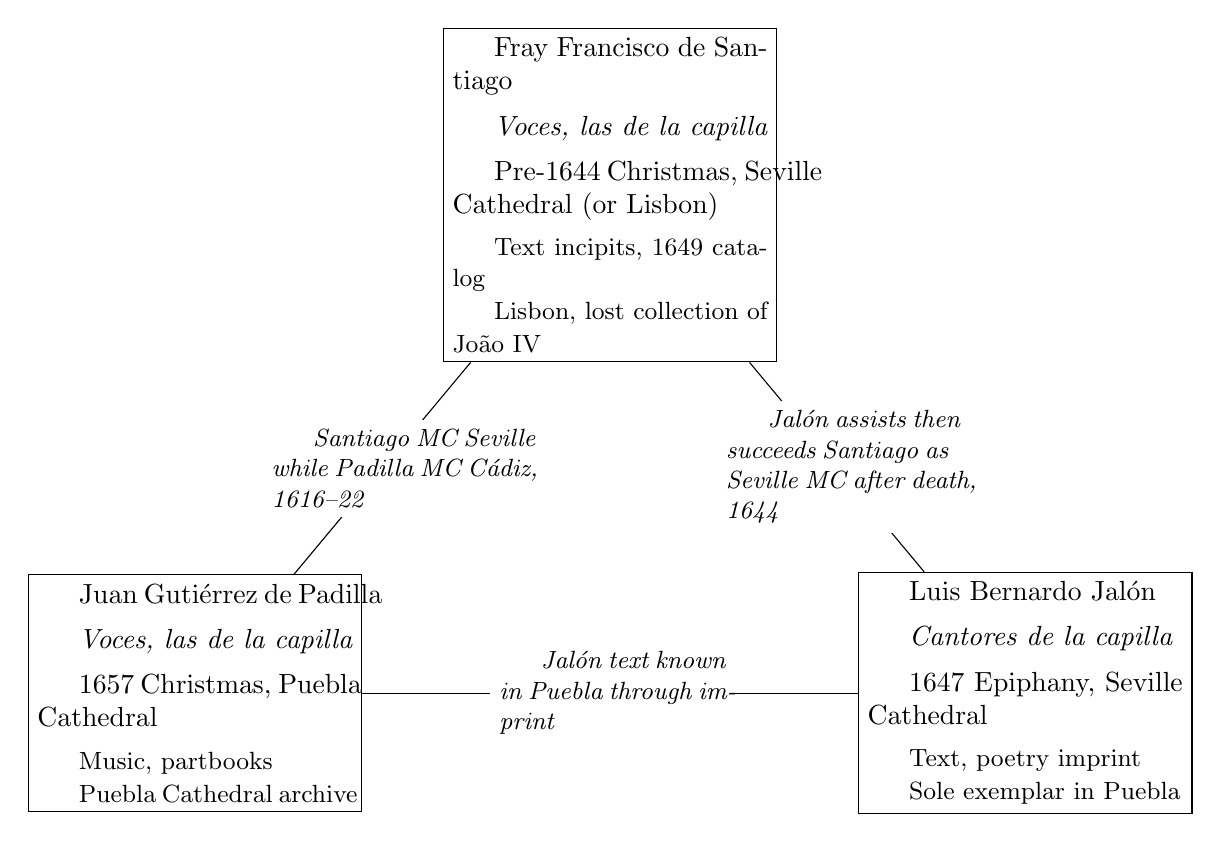
\begin{tikzpicture}[level distance=18em, 
                    sibling distance=30em,
                    every node/.style={draw},
                    edge from parent/.style={draw=none},
                    every edge quotes/.style={draw=none,fill=white}]

    \node (s) {\Santiago}
        child { node (p) {\Padilla} }
        child { node (j) {\Jalon} };
    \draw[-] (s)  edge ["\SantiagoToPadilla"  midway] (p);
    \draw[-] (s)  edge ["\SantiagoToJalon"    midway] (j);
    \draw[-] (j)  edge ["\JalonToPadilla"     midway] (p);
\end{tikzpicture}
\end{document}
